\subsection{Caso d'uso UC8: Apertura di un progetto}
\begin{figure}[h] 
	\centering 
	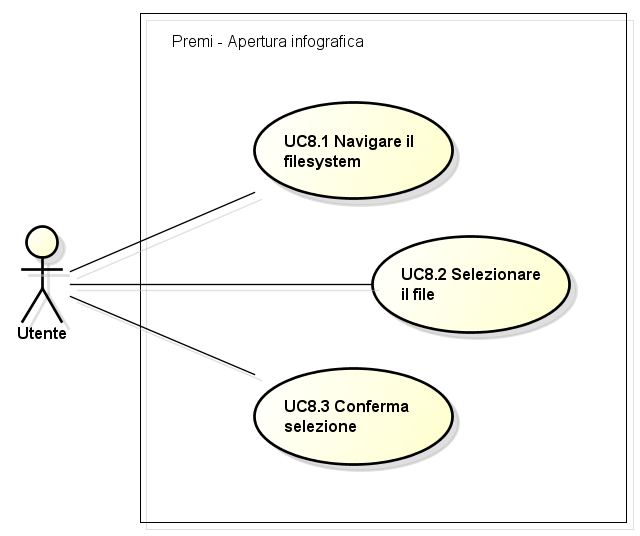
\includegraphics[width=0.7\textwidth] {img/UC8.png}
	\caption{UC8 - Apertura di un progetto} 
\end{figure}

\begin{itemize}
	\item \textbf{Attori:} Proprietario;
	\item \textbf{Scopo e descrizione:} L'utente vuole aprire un progetto esistente;
	\item \textbf{Precondizione:} L'utente si trova nella pagina che fa visualizzare i progetti disponibili;
	\item \textbf{Flusso principale degli eventi:}
	\begin{enumerate}
		\item L'utente seleziona il progetto da aprire[UC8.1].
	\end{enumerate}
	\item \textbf{Postcondizione:} Il sistema apre la schermata di modifica del progetto.
\end{itemize}


\subsubsection{Caso d'uso UC8.1: Selezionare il progetto}
\begin{itemize}
	\item \textbf{Attori:} Proprietario;
	\item \textbf{Scopo e descrizione:} L'utente seleziona il progetto che desidera aprire dalla lista dei progetti disponibili;
	\item \textbf{Precondizione:} L'utente ha selezionato un progetto già creato e salvato in precedenza;
	\item \textbf{Postcondizione:} Il sistema apre la schermata di modifica del progetto.
\end{itemize}